\chapter{Результаты исследования}

Исследование рекомендательной системы, построенной на основе алгоритма FP-Growth, использовался датасет игр с платформы Steam, содержащий 200 000 транзакций с играми, купленными пользователями.

Топ-5 самых популярных игр:
\begin{enumerate}[label*=\arabic*)]
	\item Dota 2: 4841 покупка;
	\item Team Fortress 2: 2323 покупки;
	\item Unturned: 1563 покупки;
	\item Counter-Strike Global Offensive: 1412 покупок;
	\item Half-Life 2 Lost Coast: 981 покупка.
\end{enumerate}

По извлечённым транзакциям было построено FP-дерево. В качестве начального значения параметра минимальной поддержки элемента было взято значение 0.01. На рисунке \ref{img:1} представлены самые популярные ветви построенного FP-дерева.

\begin{figure}
	\begin{center}
		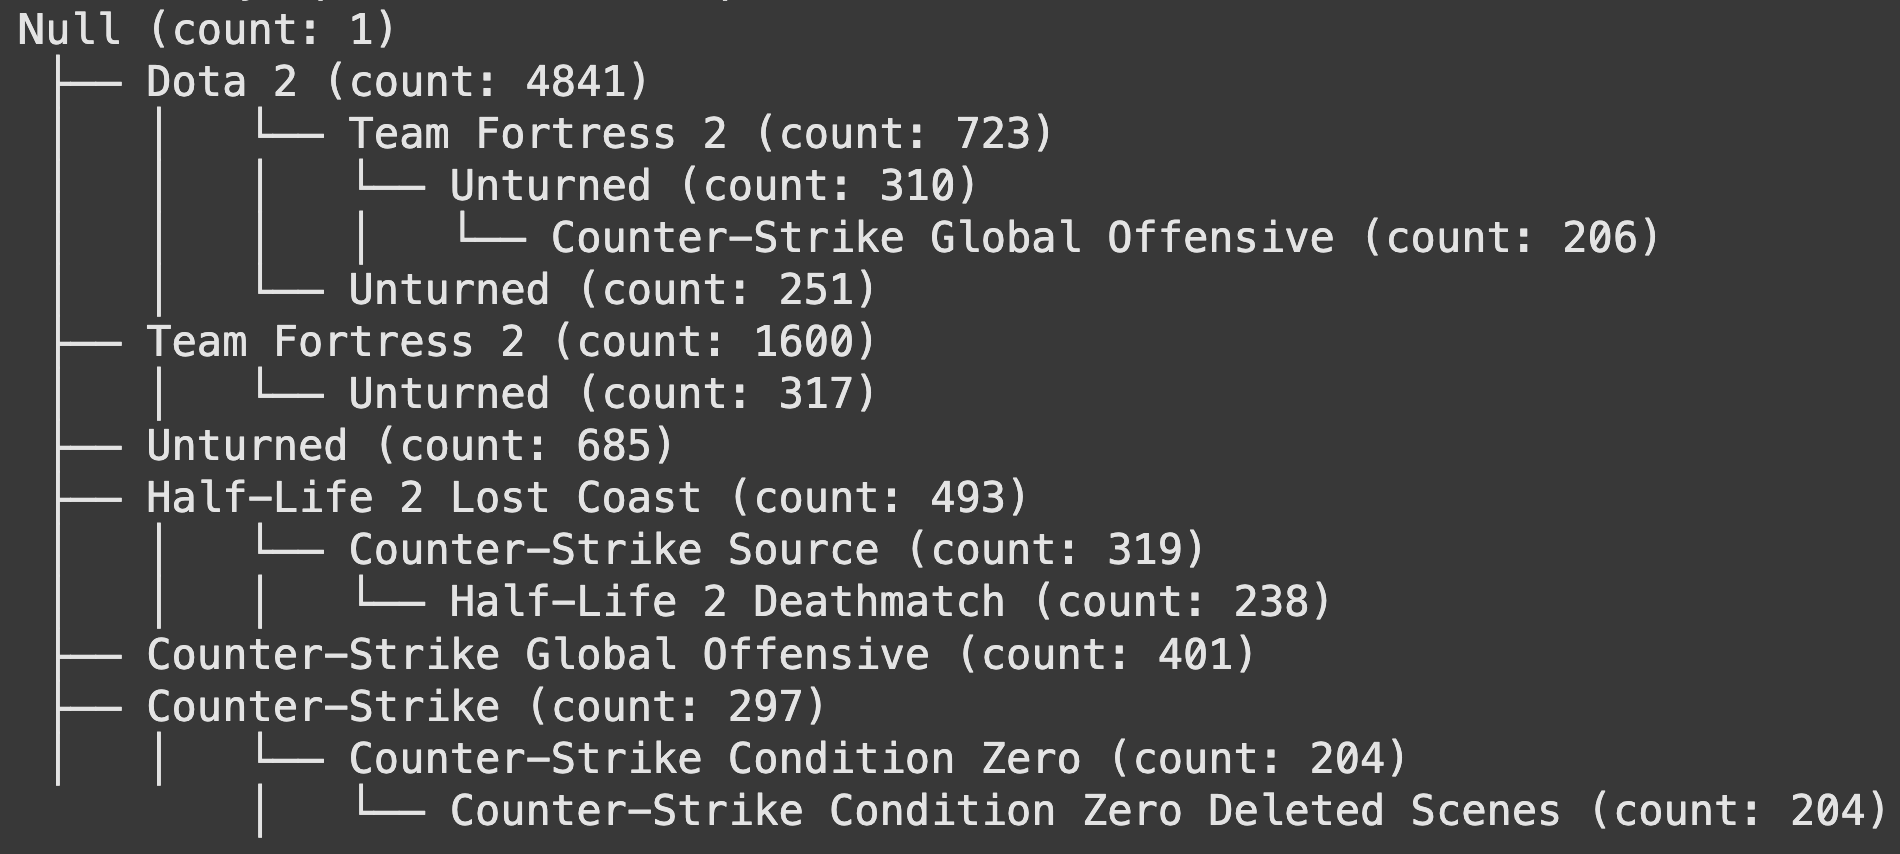
\includegraphics[width=0.9\textwidth]{images/1.png}
	\end{center}
	\caption{Самые популярные ветви FP-дерева}
	\label{img:1}
\end{figure}

Из полученного дерева были извлечены наиболее часто встречающиеся наборы объектов (1378). Каждый набор из топ-5 состоит из одного элемента и совпадает с рейтингом самых покупаемых игр.

Далее были сформированы ассоциативные правила. В качестве начального значения параметра минимальной уверенности было взято значение 0.8. 

Топ-5 правил по уверенности:
\begin{enumerate}[label*=\arabic*)]
	\item ('Magicka Vietnam') => ('Magicka') (conf: 1.0, lift: 0.00415);
	\item ('Medal of Honor Pre-Order') => ('Medal of Honor(TM) Multiplayer') (conf: 1.0, lift: 0.00885);
	\item ('Medal of Honor(TM) Multiplayer') => ('Medal of Honor Pre-Order') (conf: 1.0, lift: 0.00885);
	\item ('Medal of Honor Pre-Order') => ('Medal of Honor(TM) Single Player') (conf: 1.0, lift: 0.00885);
	\item ('Medal of Honor(TM) Single Player') => ('Medal of Honor Pre-Order') (conf: 1.0, lift: 0.00885).
\end{enumerate}

Рейтинг полученных правил не соответствует рейтингу самых покупаемых игр.

Для определения оптимальных настроечных значений параметров реализованный алгоритм был запущен с диапазоном минимальной поддержки от 0.005 до 0.025 с шагом 0.025 и минимальной уверенности от 0.65 до 0.975 с шагом 0.025. На рисунках \ref{img:2}-\ref{img:5} представлены результаты исследования характеристик наборов правил, полученных при различных значениях настроечных параметров.

\begin{figure}
	\begin{center}
		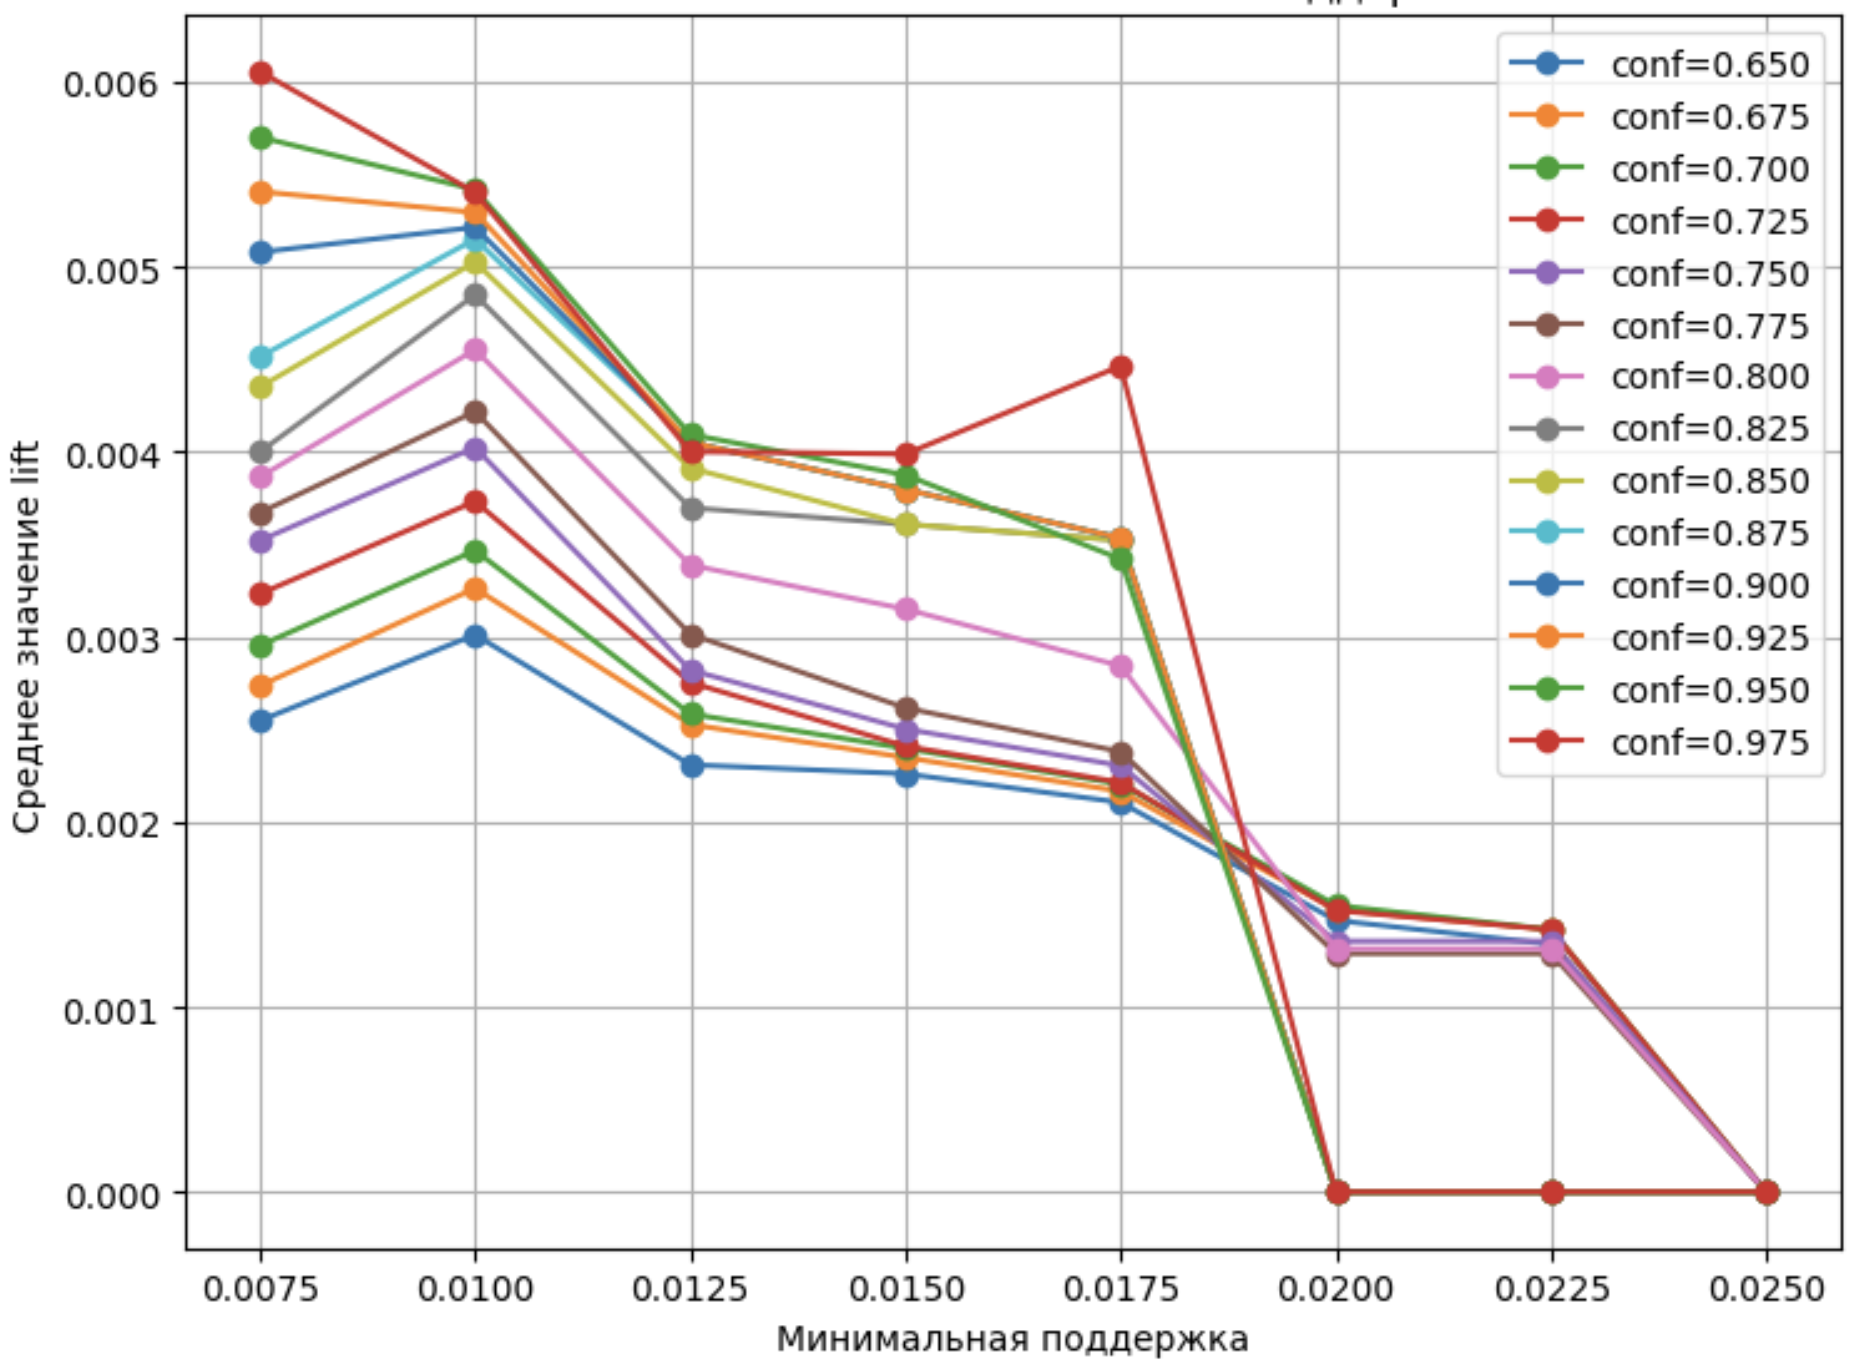
\includegraphics[width=0.95\textwidth]{images/2.png}
	\end{center}
	\caption{Зависимость lift от минимальной поддержки}
	\label{img:2}
\end{figure}

\begin{figure}
	\begin{center}
		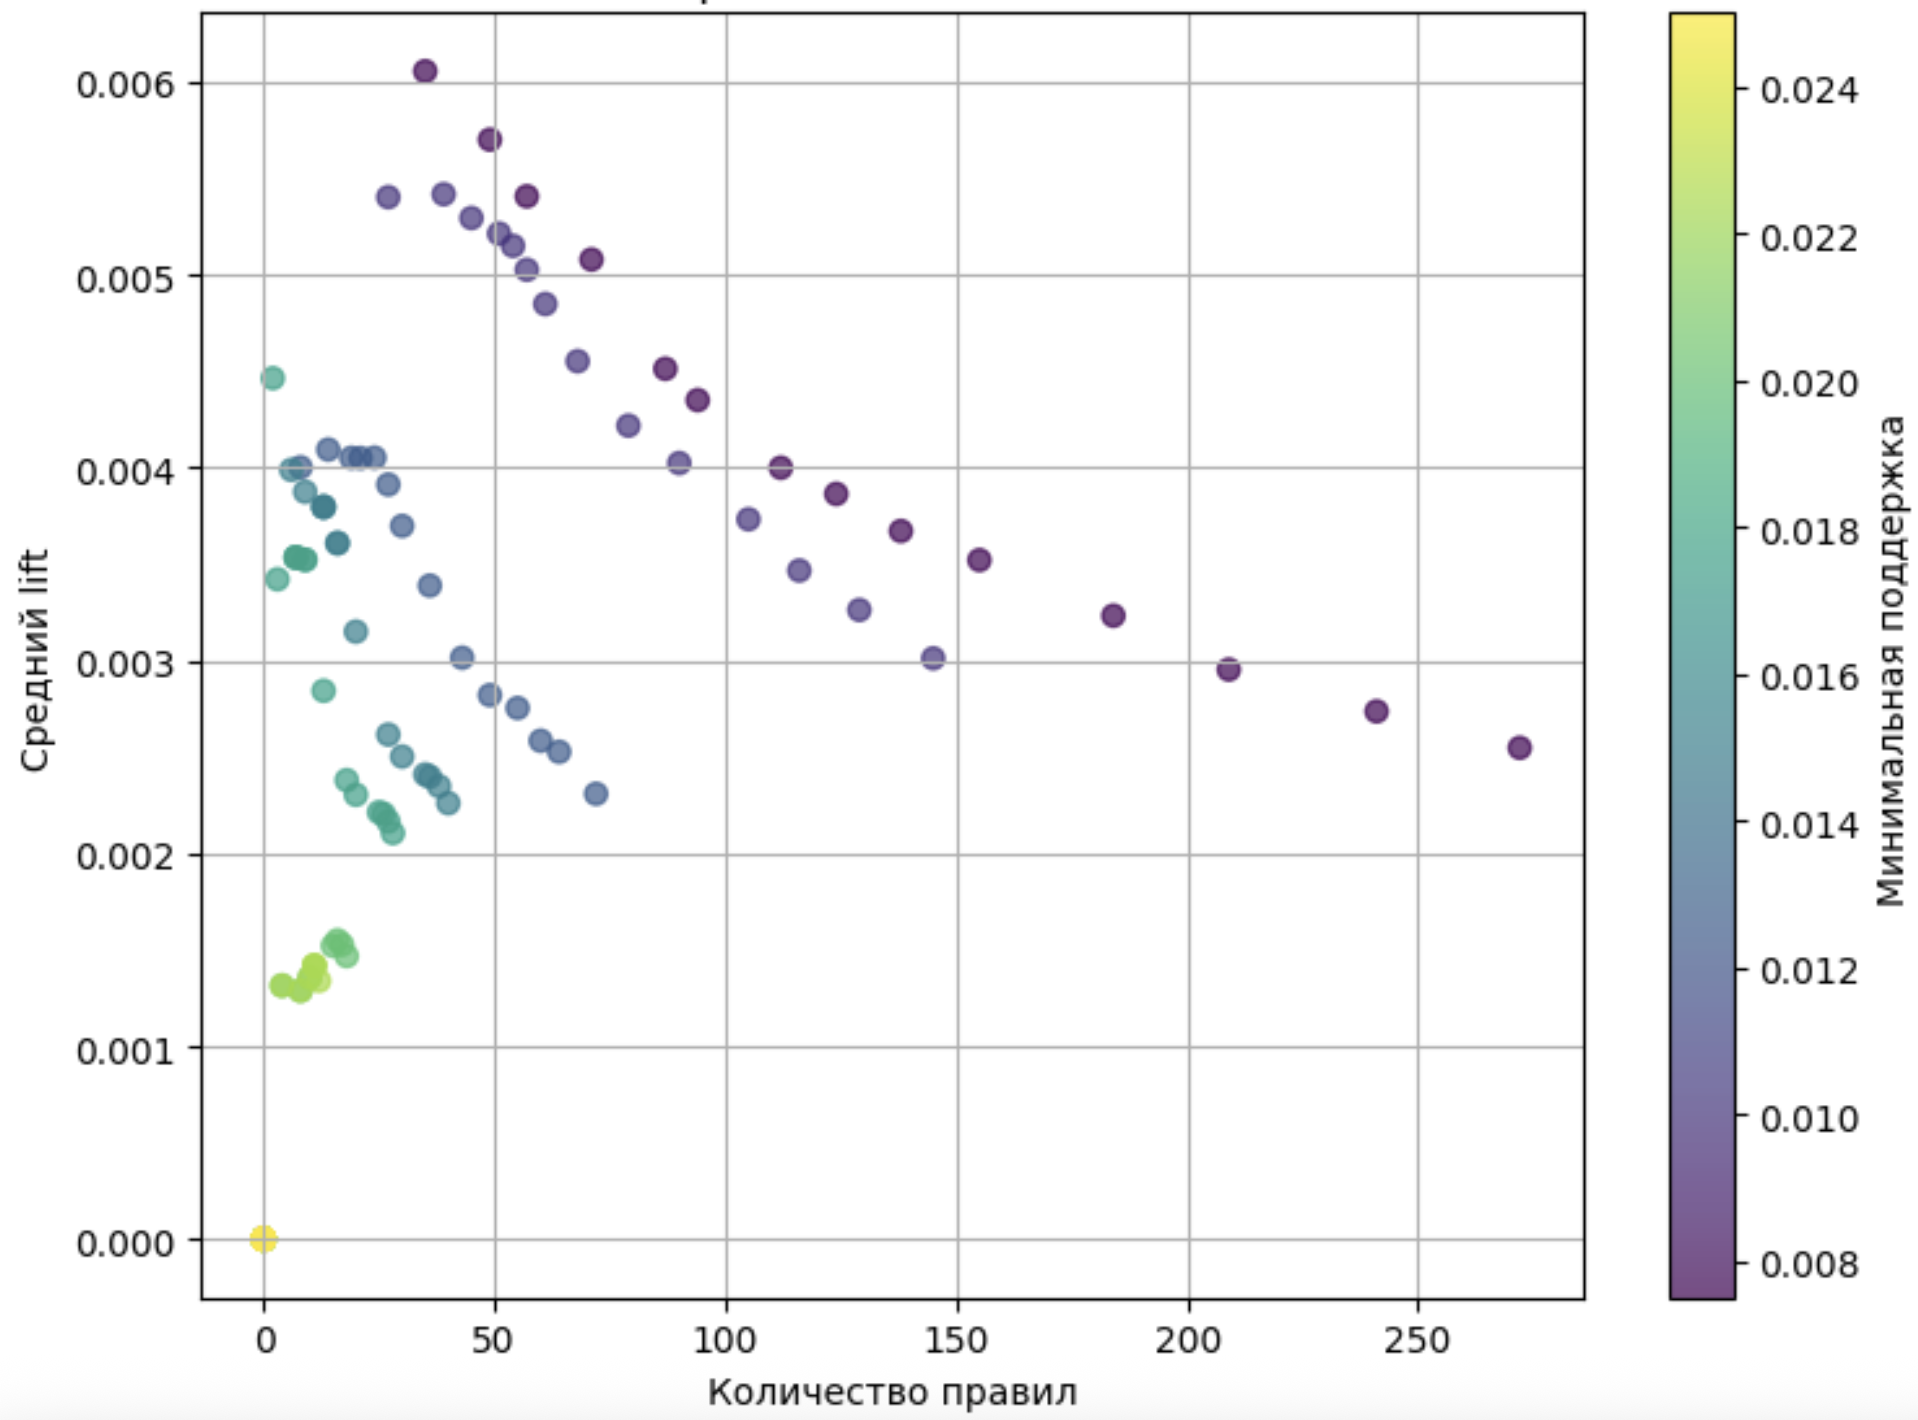
\includegraphics[width=\textwidth]{images/3.png}
	\end{center}
	\caption{Зависимость количества правил и lift от минимальной поддержки при различных значениях минимальной уверенности}
	\label{img:3}
\end{figure}

\begin{figure}
	\begin{center}
		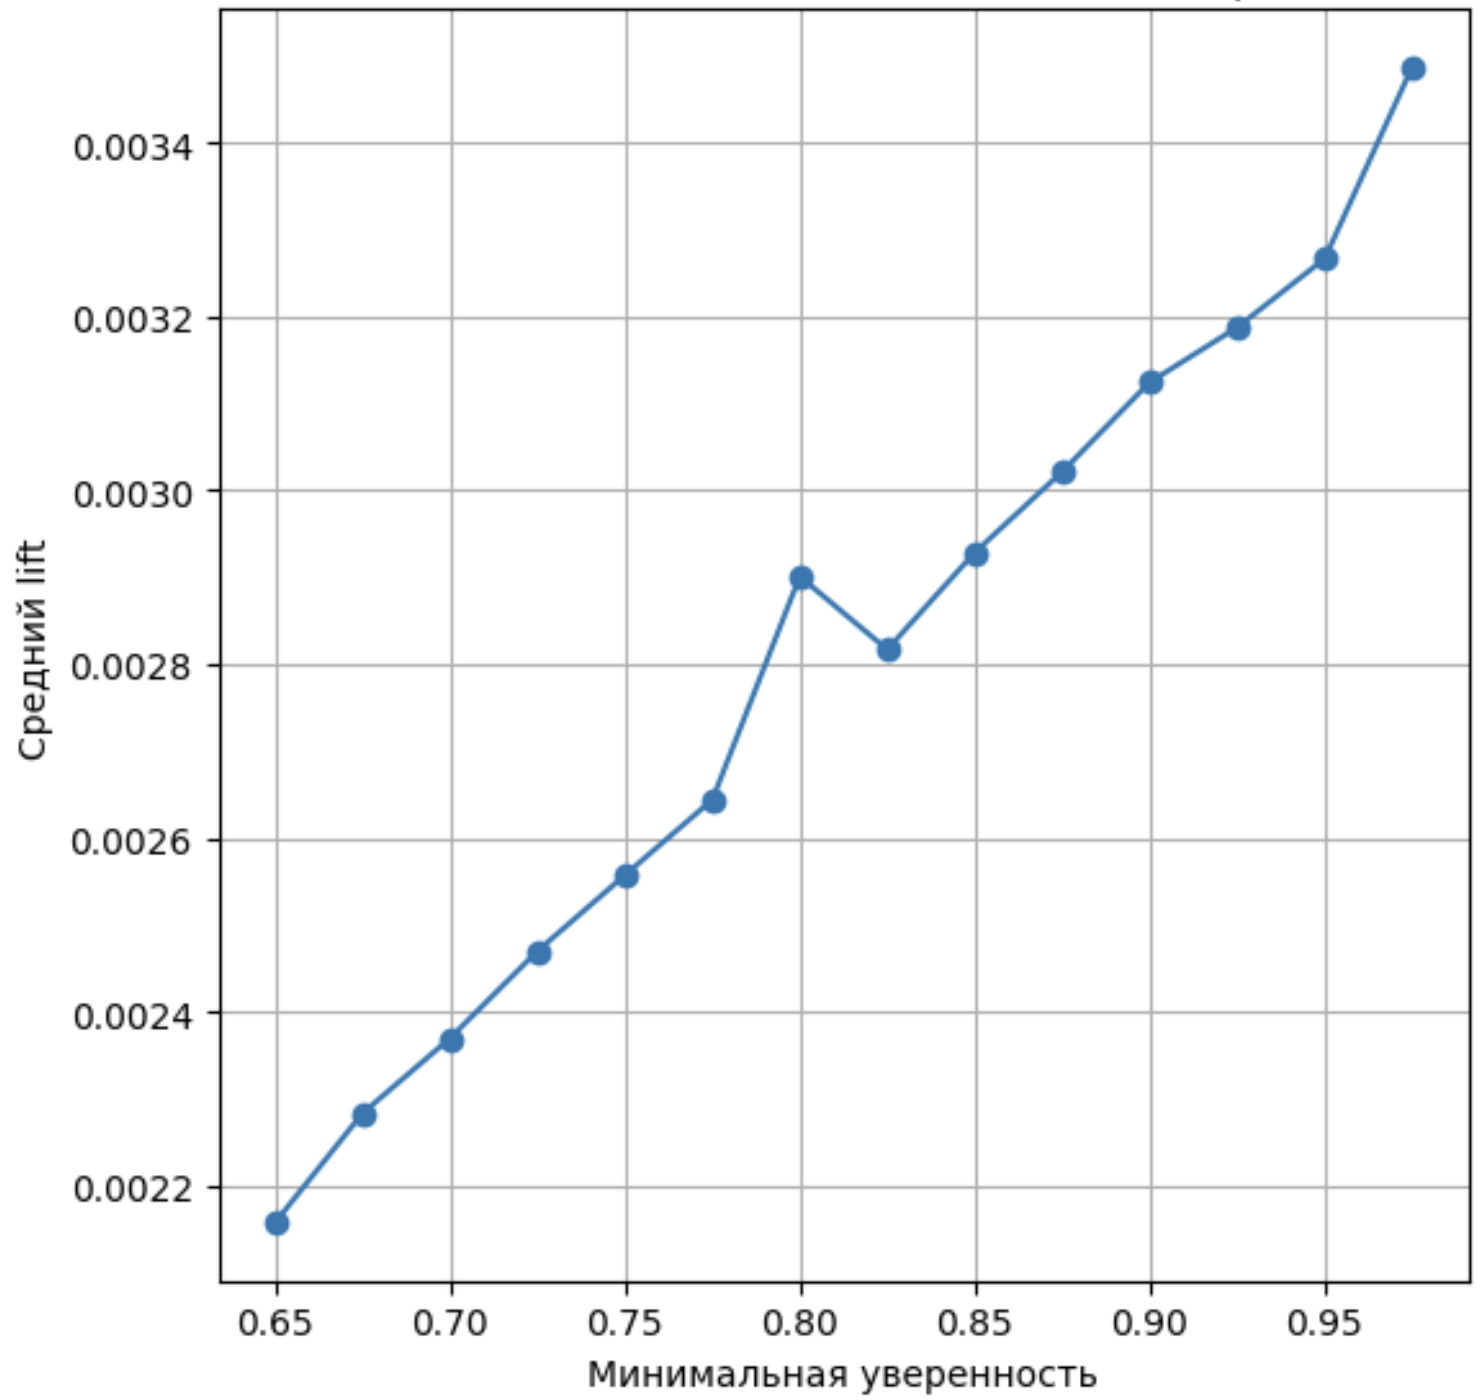
\includegraphics[width=0.7\textwidth]{images/4.png}
	\end{center}
	\caption{Зависимость lift от минимальной уверенности}
	\label{img:4}
\end{figure}

\begin{figure}
	\begin{center}
		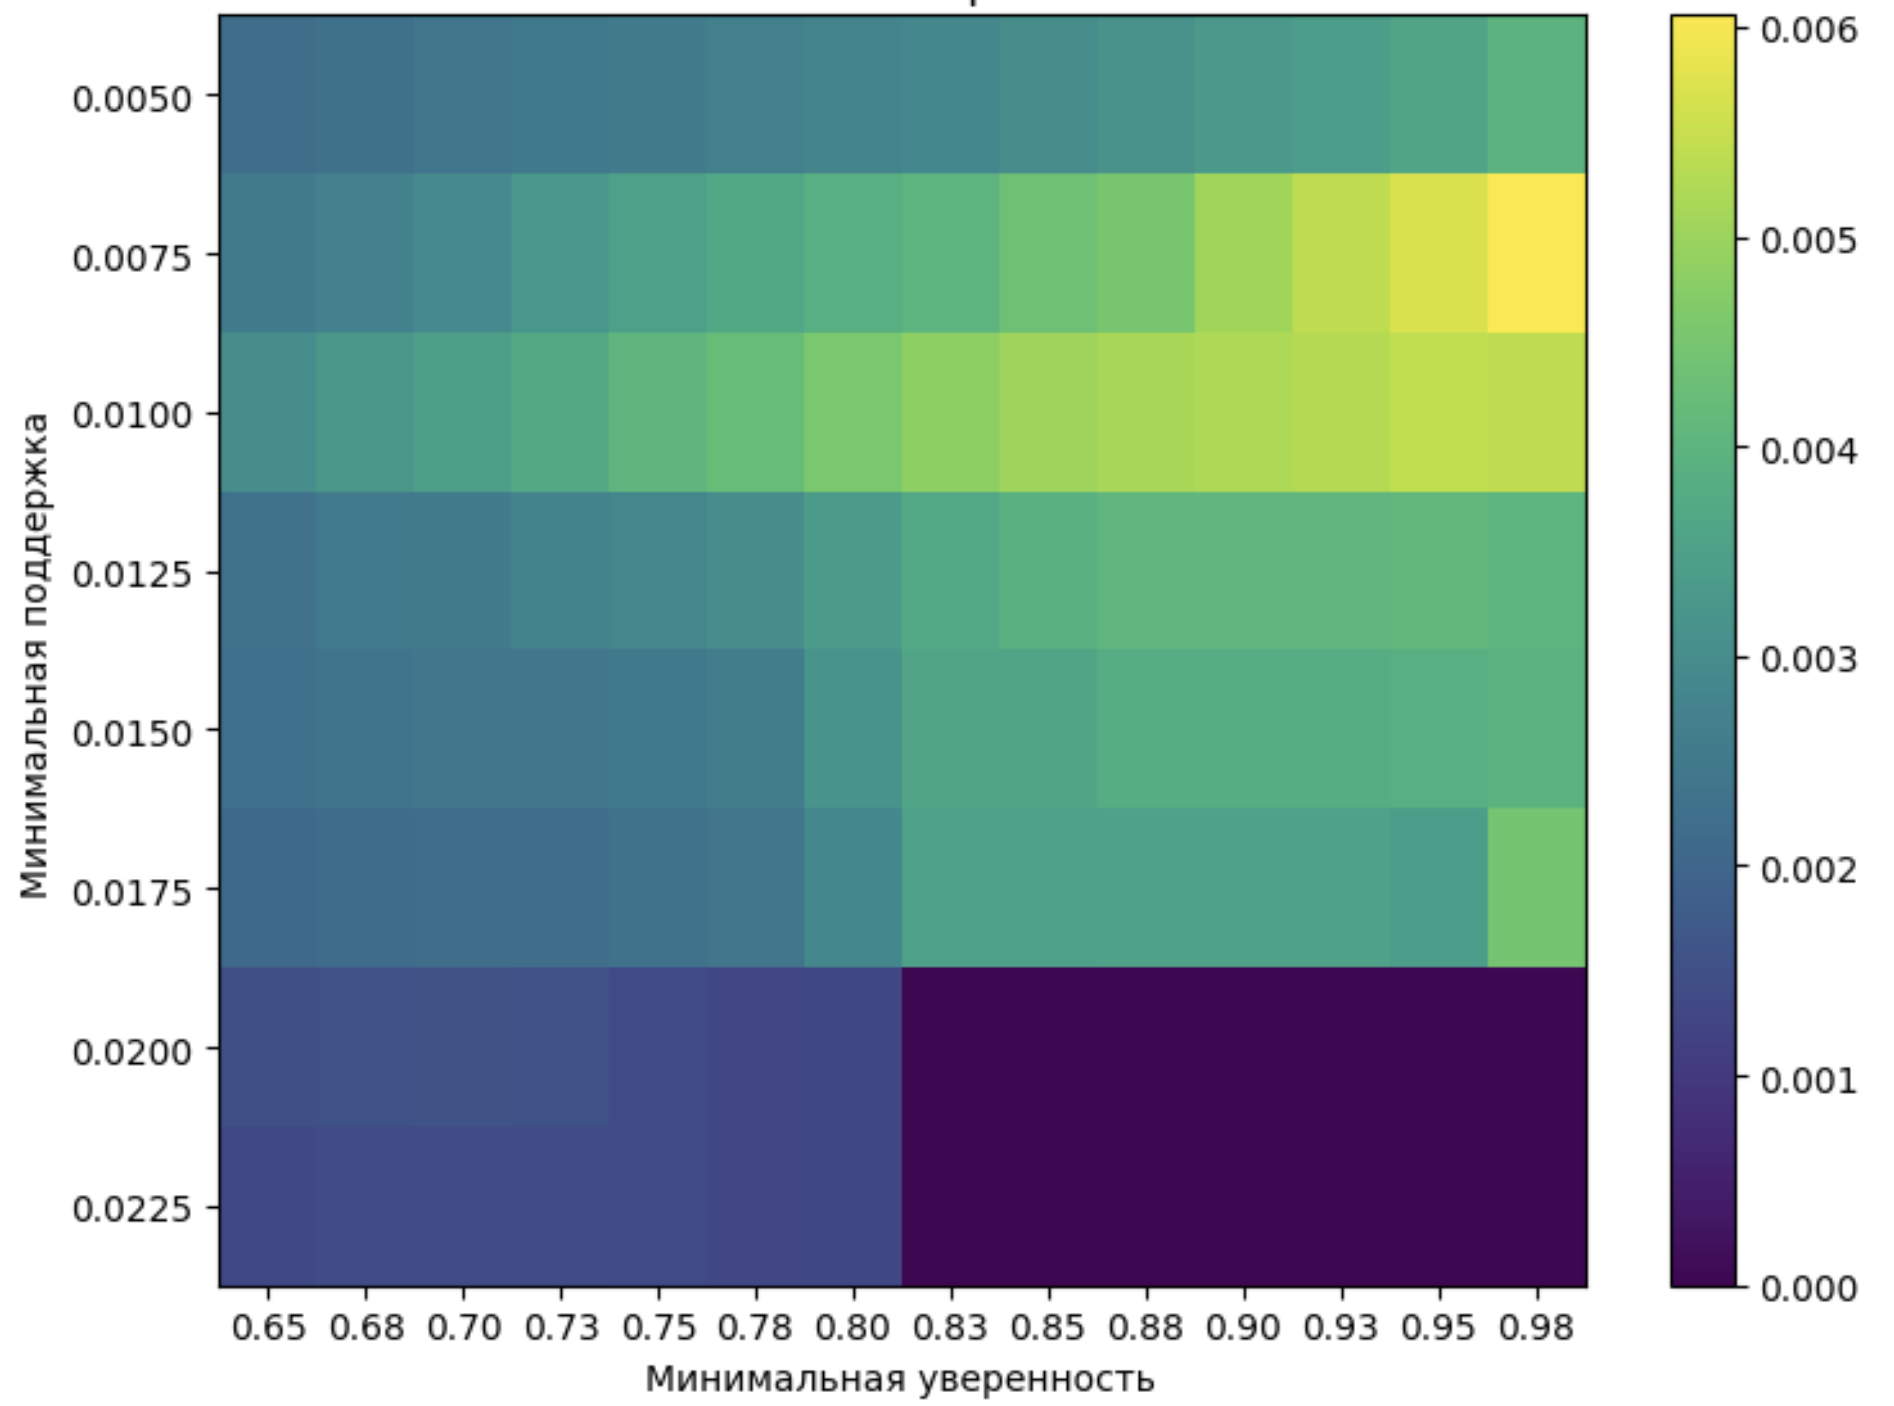
\includegraphics[width=0.7\textwidth]{images/5.png}
	\end{center}
	\caption{Тепловая карта значений lift}
	\label{img:5}
\end{figure}

\clearpage
